\subsection{Layout \& Design}

Die App besteht grundsätzlich aus drei Bereichen:
einer Liste, einem Informations-Panel und einem Formular.
Diese Bereiche sollen nahtlos ineinander übergehen um ein
möglichst professionellen Gesamteindruck zu vermitteln.
Das finale Layout entspricht in der Hauptansicht der untenstehenden Abbildung.

\begin{figure}[H]
    \minipage[t]{0.4\textwidth}\vspace{0pt}
        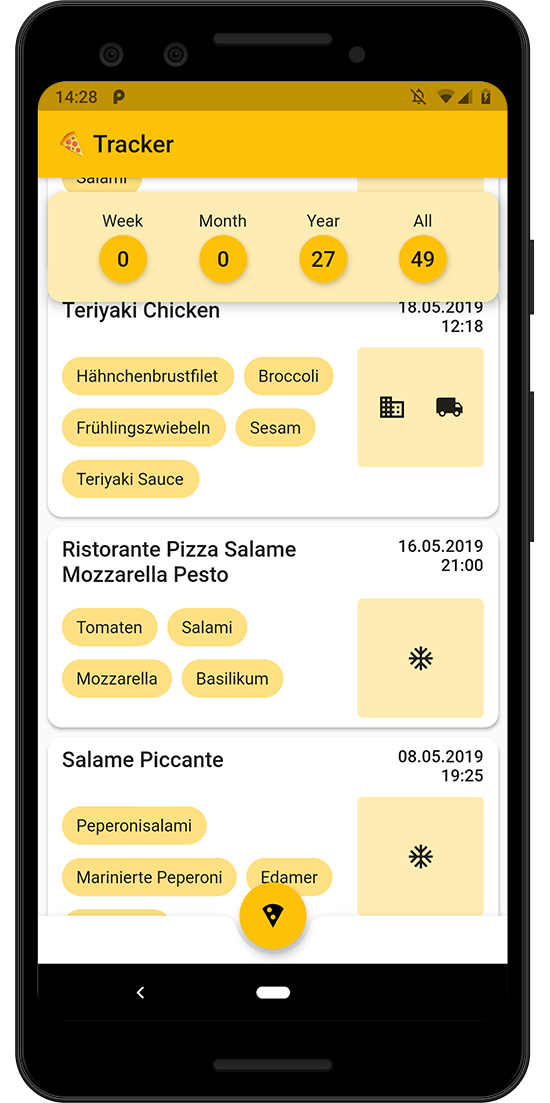
\includegraphics[width=\linewidth]{pixel-3_mockup-1}
        \caption{
            App: Hauptansicht
        }
    \endminipage\hfill
    \minipage[t]{0.6\textwidth}\vspace{0pt}
        Die Anordnung von Elementen erfolgt bei Flutter wie im Web:
        Die Reihenfolge im Quellcode gibt zugleich deren Reihenfolge auf
        der Y-Achse an. Elemente können sich dabei (auf der Z-Achse)
        nicht überlagern. Um Elemente übereinander darzustellen gibt es
        im Web die Property \textit{z-index}, in Flutter nutzt man das Widget
        \textit{Stack}. Im Stack-Widget ist das erste Element das auf der
        Z-Achse niedrigste Element. Grundsätzlich lassen sich viele
        Layout-Konzepte aus dem Web in Flutter übertragen. So gibt es
        Widgets wie \textit{Row, Column, Grid, Flex und Expanded} welche
        in ihrer Funktionalität gleich ihren Web-Pendants entsprechen.
        Interessant ist, dass \textit{Row} allerdings nicht umbricht,
        sobald zu viele Elemente in einer Zeile vorhanden sind und man
        für diesen Fall das Widget \textit{Wrap} benutzen muss.
        Grundsätzlich bietet Flutter eine große Auswahl an Widgets, die über
        reine Layout-Funktionalitäten hinaus gehen und optische Standardwerte
        mit sich bringen. So gibt es das \textit{Card}-Widget welches über
        dessen Properties \textit{elevation} und \textit{shape} einfache
        Mittel bereitstellt, um die Material-Design-typischen Schatten
        und abgerundeten Ecken zu erzielen.

    \endminipage\hfill
\end{figure}
Um nicht nur am oberen, sondern auch am unteren Ende der App
(am sogenannten \ac{FAB}) ein \textit{Überfließen} zu erzielen,
muss die Fläche der Liste auf die komplette Höhe des
Bildschirms erweitert werden.

\begin{figure}[H]
    \minipage[t]{0.4\textwidth}\vspace{0pt}
        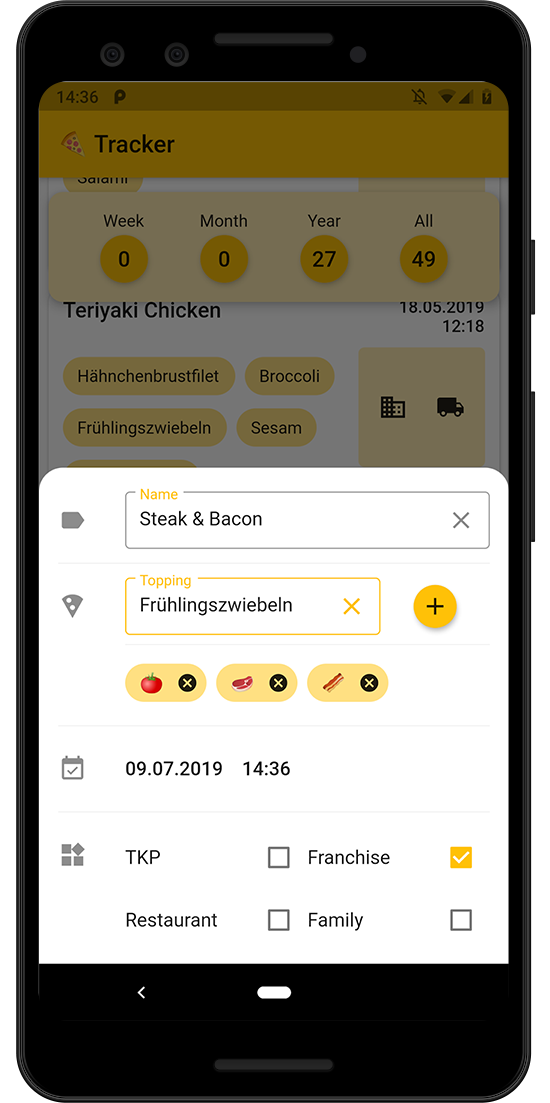
\includegraphics[width=\linewidth]{pixel-3_mockup-2--form}
        \caption{
            App: Formular
        }
    \endminipage\hfill
    \minipage[t]{0.6\textwidth}\vspace{0pt}
        Das Formular an sich besteht mehreren, grundsätzlich
        unabhängigen, Widgets:

        \begin{itemize}
            \itemsep-0.4em
            \item Name
            \item Toppings
            \item Datum \& Uhrzeit
            \item Art der Pizza:
            \begin{itemize}
                \itemsep-0.4em
                \item \ac{TKP}
                \item Franchise
                \item Restaurant
                \item Family
                \item Delivery
                \item Selfmade
            \end{itemize}
            \item Ort an dem die Pizza gegessen wurde
        \end{itemize}

        Hierbei stellten sich vor allem die Widgets für die
        Eingabe der Toppings und der Art der Pizza als besonders
        anspruchsvoll heraus. Bei den Toppings kam zum einen
        zwei Mal das \textit{Row}-, ein Mal das \textit{Wrap}
        sowie für die Toppings selbst das \textit{Chip}-
        (mit \textit{onDeleted}-Methode), bei der
        Art der Pizza vor allem das \textit{Grid}- sowie
        das \textit{Checkbox}- (in Kombination) mit dem \textit{Text}-Widget
        zum Einsatz.
    \endminipage\hfill
\end{figure}
Um im Formular abgerundete Ecken darstellen zu können, benötigt man
das extern erhältliche Widget \textit{showRoundedModalBottomSheet}.
Allerdings kann auch dieses nicht über eine Höhe von 50\% des Bildschirms
hinaus gehen und zwingt einen somit zum scrollen.

\begin{figure}[H]
    \centering
    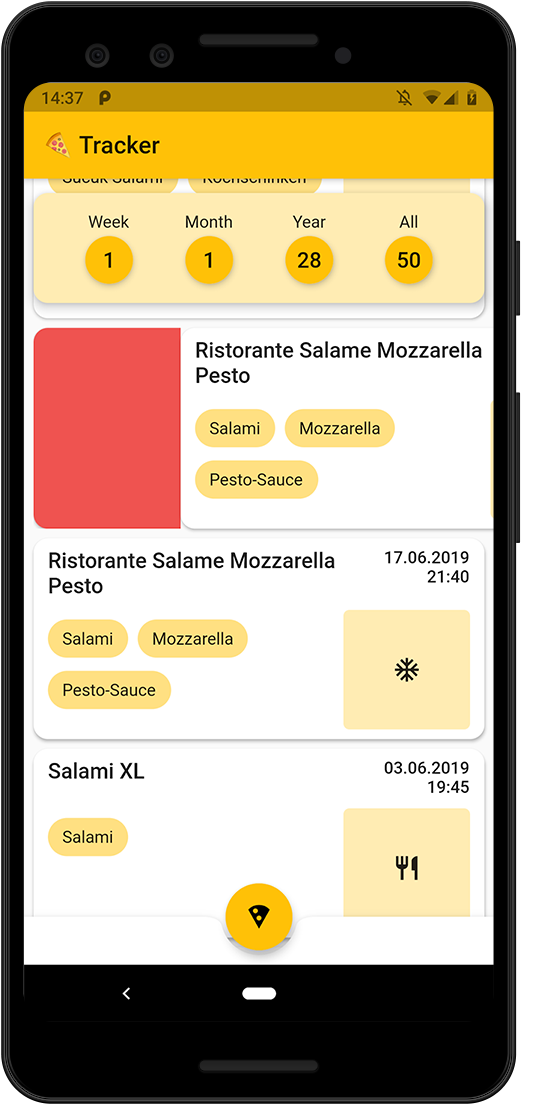
\includegraphics[width=0.4\columnwidth]{pixel-3_mockup-3--dismissible}
    \caption{App: Dismissible}
\end{figure}

Um Pizzen schnell wieder löschen (und später potentiell bearbeiten)
zu können, bietet sich das \textit{Dismissible}-Widget an.
Dieses kann man beliebig um andere Widgets packen und diesem
durch wischen in bestimmte Richtungen verschiedene Aktionen zuweisen.
\newpage
